\documentclass[UTF8,a4paper,11pt,fontset=windows]{ctexart}
\usepackage[margin=2.1cm]{geometry}
\usepackage{graphicx,float,booktabs,tabularx,fancyhdr,xurl,fvextra}
\usepackage[hidelinks]{hyperref}
\setlength{\parskip}{.25em}
\setlength{\emergencystretch}{2em}
\renewcommand{\arraystretch}{1.2}
\pagestyle{fancy}\fancyhf{}
\fancyhead[L]{互联网数据库开发 · 知行学习团队}
\fancyhead[R]{2413581 黄奕浩}\fancyfoot[C]{\thepage}
\setlength{\headheight}{14pt}\raggedbottom
\begin{document}
\begin{titlepage}\thispagestyle{empty}\centering
\vspace*{.6cm}
\includegraphics[width=.43\textwidth]{../../figures/nankai_logo_color.png}
\vspace{.9cm}\rule{.88\textwidth}{.8pt}\par\vspace{.55cm}
{\fontsize{27pt}{35pt}\selectfont\bfseries 互联网数据库开发课程设计\par}
\vspace{.65cm}{\fontsize{21pt}{29pt}\selectfont\bfseries 实现文档\par}
\vspace{.55cm}\rule{.88\textwidth}{.8pt}\par
\vspace{1.3cm}{\Large 知行学习团队\par}
\vspace{.6cm}{\large 黄奕浩\quad 2413581\quad 组长\par
王乐之\quad 2411302\par 黄乐仁\quad 2413628\par}
\end{titlepage}
\section{公共模块与MVC调用}
本人负责包含登录注册、团队及成员展示、后台资料维护、公告发布与作业下载。公共Model封装数据约束，Controller检查身份与处理请求，View只负责显示转义后的内容和表单。以成员展示为例，MemberController查询MemberProfile后传给详情视图，后台修改同一记录，因此前台刷新即可读取更新后的介绍。

\section{账户与权限}
普通注册账户固定为member角色，密码经Yii安全组件生成哈希。后台登录额外检查admin角色，并对整个后台应用应用访问控制。成员编辑动作从当前登录会话确定记录，不使用请求里的用户ID定位编辑目标。site/me提供其他两位模块可复用的身份接口。

\section{团队首页与成员维护}
首页采用深绿导航、浅色介绍区与成员卡片组织内容，页面读取数据库中的团队介绍、成员资料和最新公告。三位成员的分工用简短介绍展示。后台提供团队介绍表单、成员列表和编辑表单，字段包含姓名、学号与介绍。

\begin{figure}[H]\centering
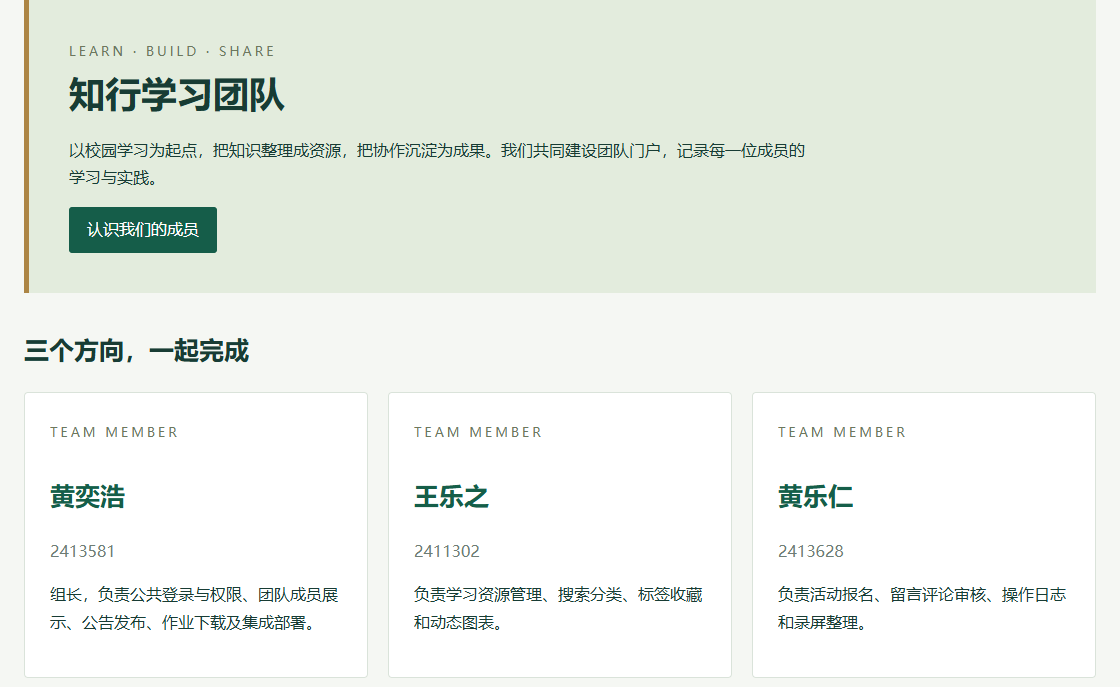
\includegraphics[width=\linewidth,height=.40\textheight,keepaspectratio]{../../figures/01-首页.png}
\caption{团队首页与成员分工展示}
\end{figure}

\begin{figure}[H]\centering
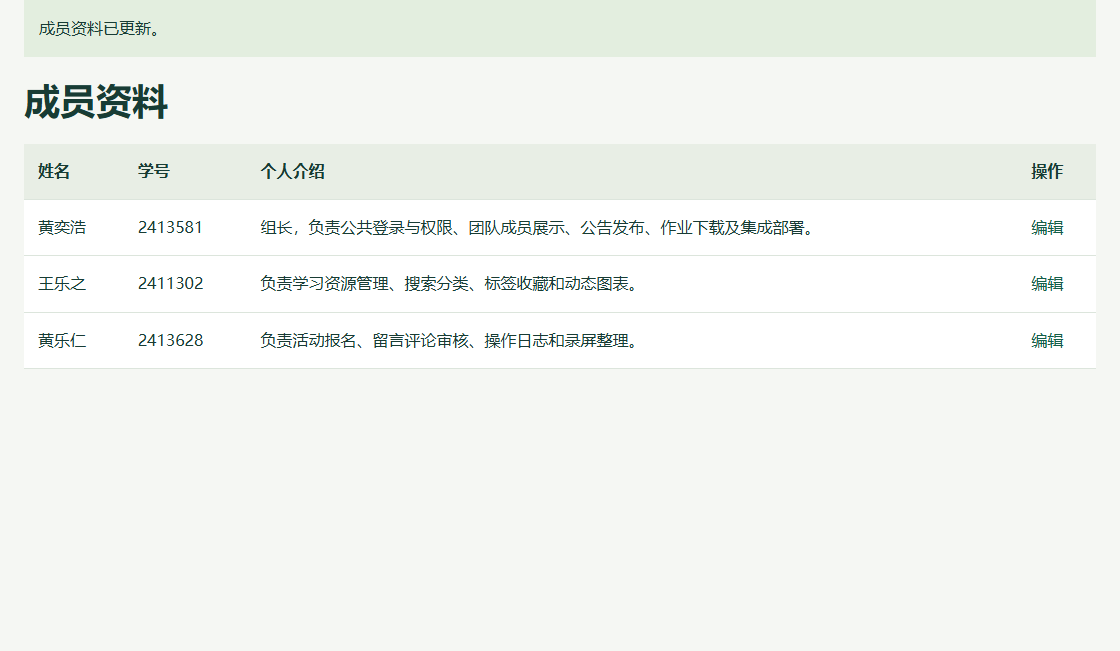
\includegraphics[width=\linewidth,height=.33\textheight,keepaspectratio]{../../figures/03-成员管理.png}
\caption{后台成员维护}
\end{figure}
\section{公告发布与内容处理}
Announcement模型定义标题长度、内容长度和三种状态；管理员表单只加载允许编辑的字段，作者由服务器会话设置。发布时写入发布时间，草稿和撤下状态不会出现在前台查询中。删除使用POST并校验CSRF令牌。公告正文按普通文本展示，因此输入HTML标签只会显示文本，不会执行脚本。

\begin{figure}[H]\centering
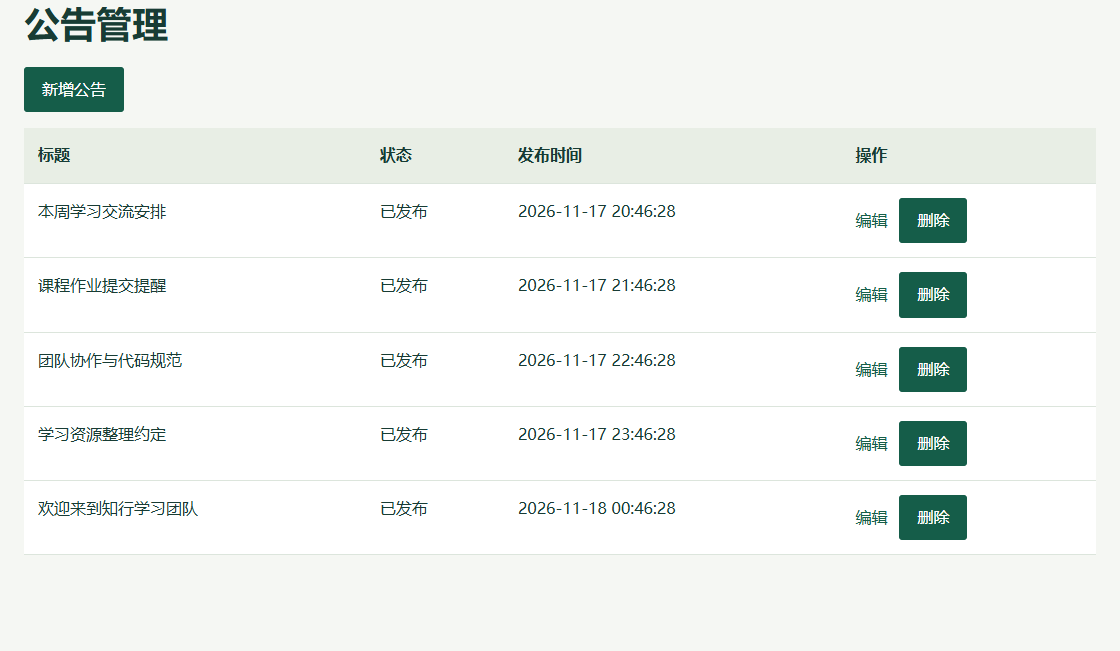
\includegraphics[width=\linewidth,height=.33\textheight,keepaspectratio]{../../figures/05-公告管理.png}
\caption{公告状态与管理操作}
\end{figure}
\section{作业文件下载}
AssignmentFile保存文件类别、相对路径和SHA256。下载动作仅接收记录编号，不接受任意文件路径。模型限定team或personal目录，解析真实路径并检查是否仍处于data目录，随后验证文件摘要。缺失或不一致的文件不提供下载按钮，直接请求返回404。当前接入本人的三份个人作业及已经整理的团队材料。

\begin{figure}[H]\centering
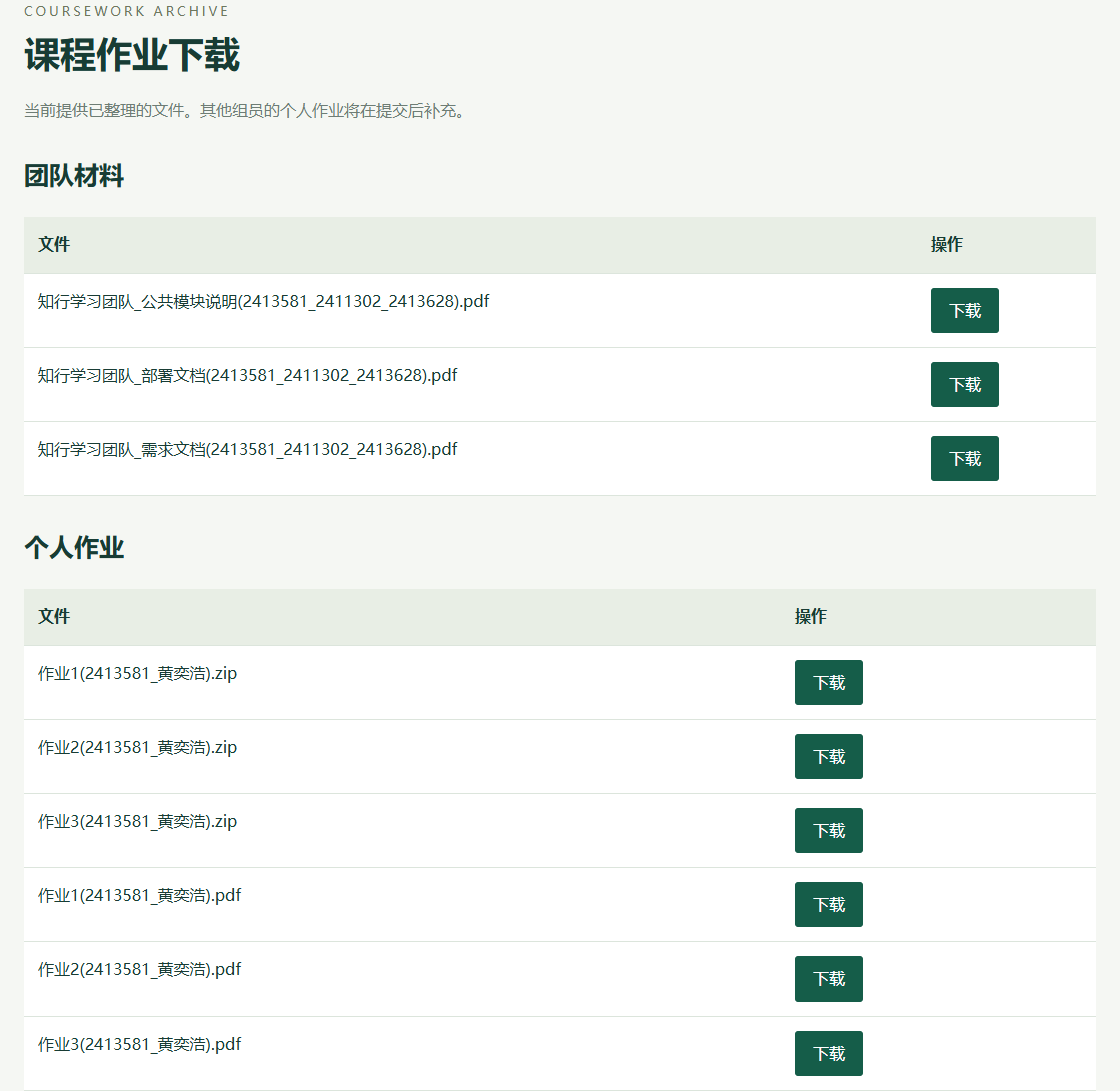
\includegraphics[width=\linewidth,height=.33\textheight,keepaspectratio]{../../figures/06-作业下载.png}
\caption{团队材料与个人作业下载}
\end{figure}
\section{交接接口}
王乐之可在资源发布、收藏等动作中使用Yii当前会话身份和site/me返回的用户编号，所有权需在对应模块服务器端检查。黄乐仁可在报名和留言中引用user主键。公共布局与Model保持独立，资源和活动模块可以新增导航入口，不需要修改已经完成的身份与下载逻辑。

当前演示使用三条成员资料和五条自拟公告。其他两位负责的资源、活动、留言和日志尚未接入，不以公共模块的页面截图代替他们的实现成果。
\section{协作记录、主要代码与目录}
Git记录取自实际仓库的git log，主要代码及目录截图来自实际源文件和受控文件清单，使用浏览器只读展示而非伪装成终端。任务分工已写入成员MD；Tower截图待登录完成真实任务操作后补入，步骤见截图采集说明。

\begin{figure}[H]\centering
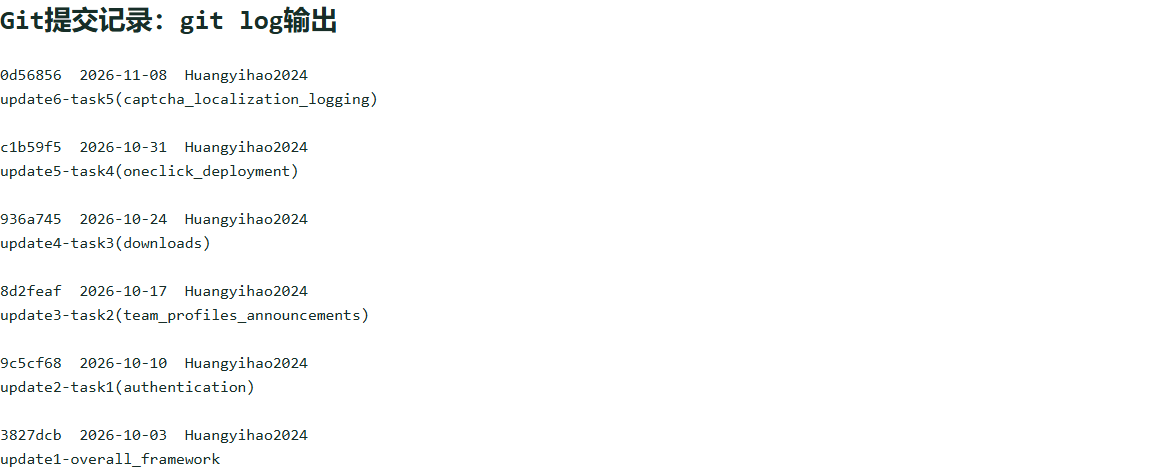
\includegraphics[width=\linewidth,height=.33\textheight,keepaspectratio]{../../figures/git_history.png}
\caption{实际Git提交记录}
\end{figure}

\begin{figure}[H]\centering
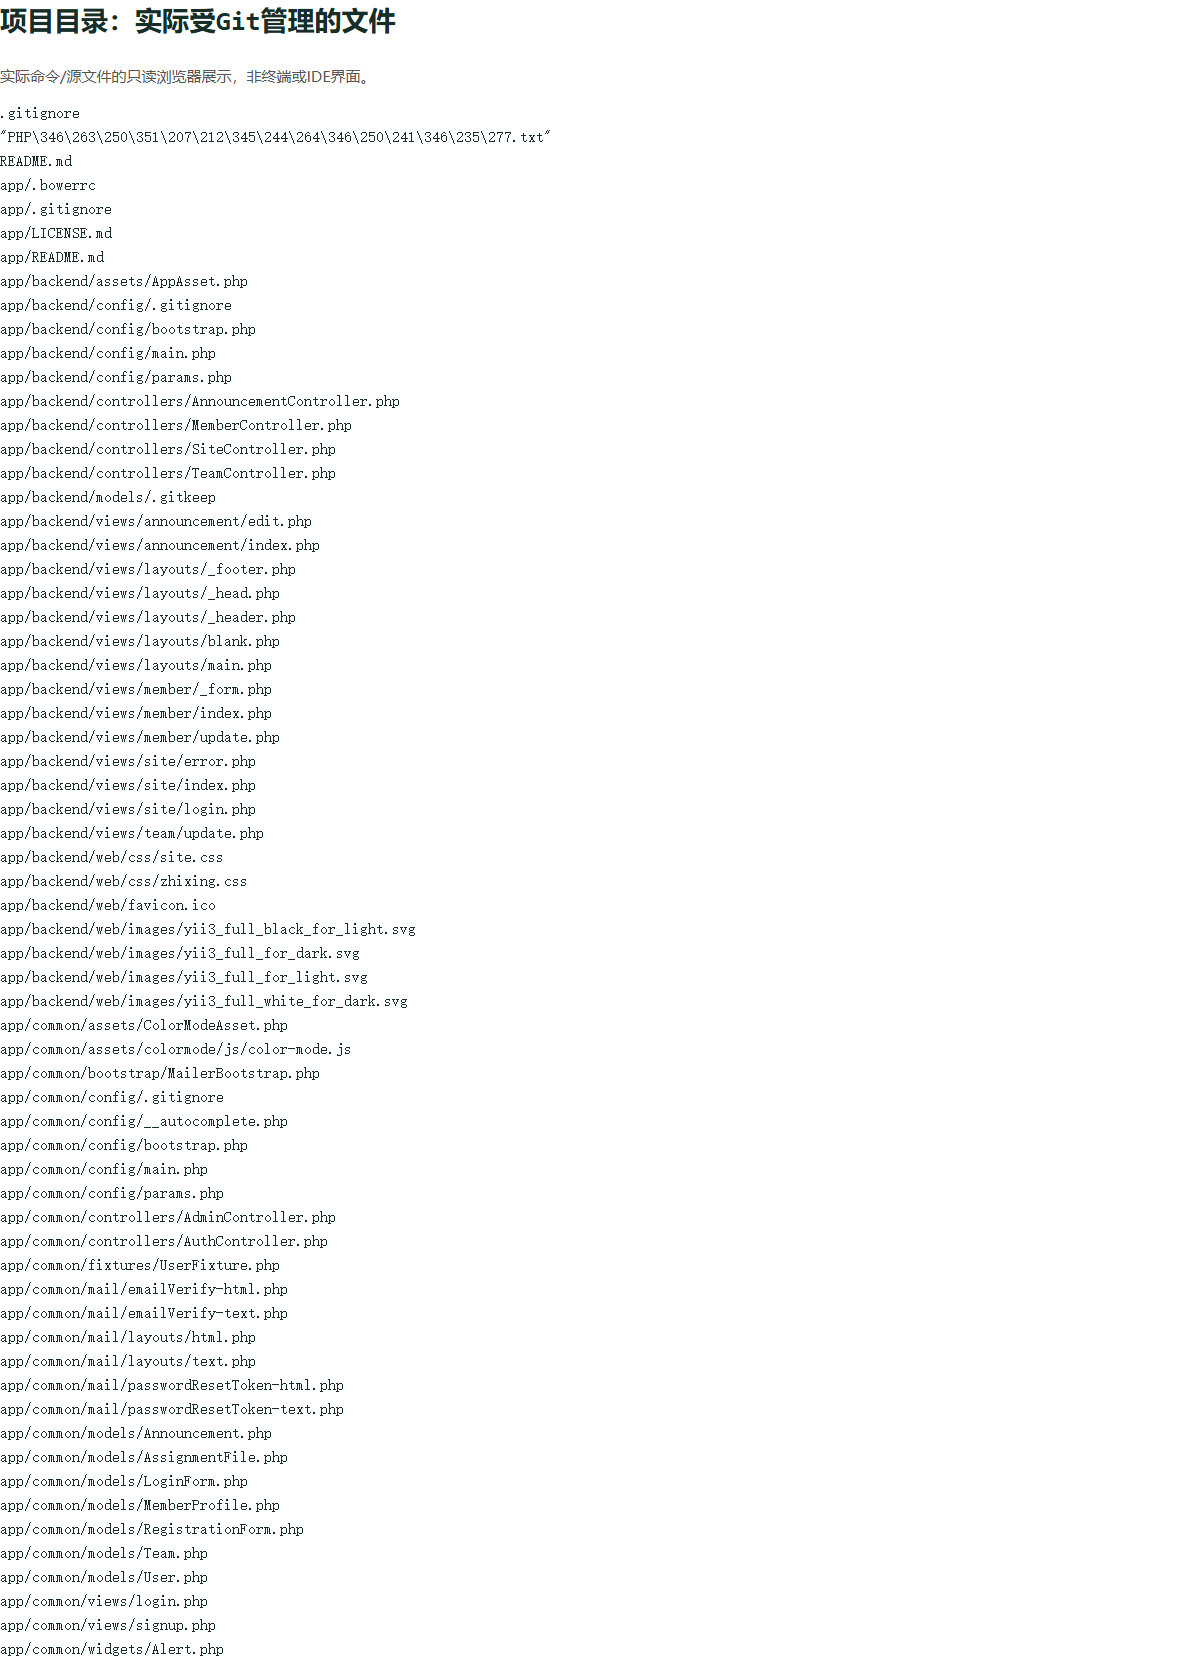
\includegraphics[width=\linewidth,height=.33\textheight,keepaspectratio]{../../figures/source_tree.png}
\caption{受控项目目录}
\end{figure}

\begin{figure}[H]\centering
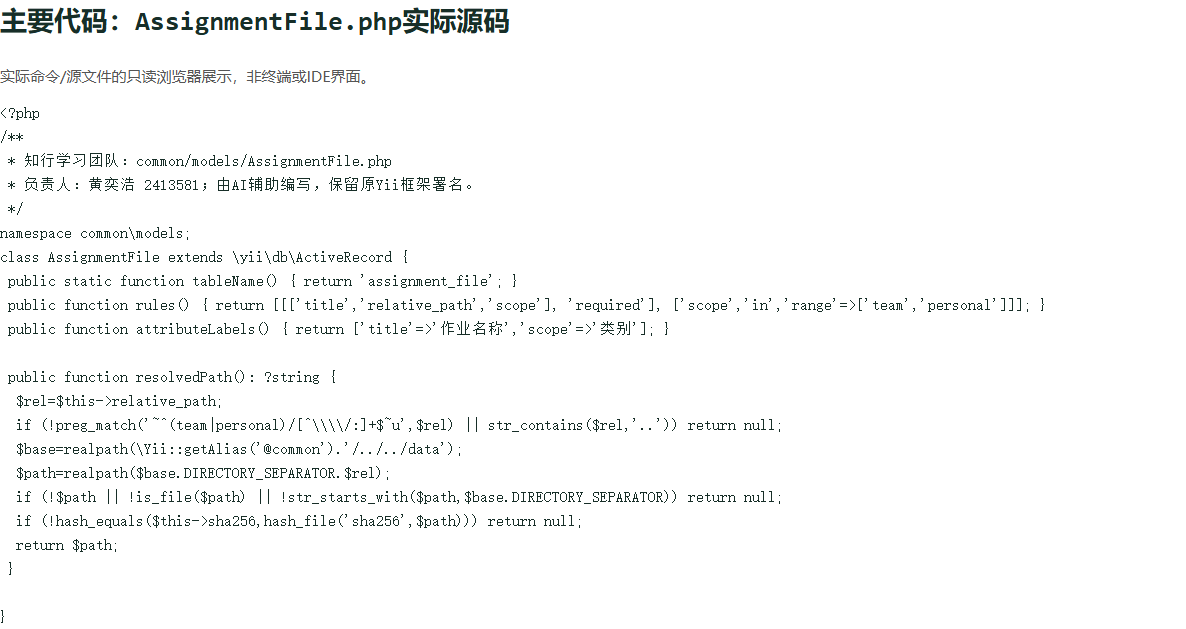
\includegraphics[width=\linewidth,height=.33\textheight,keepaspectratio]{../../figures/source_code.png}
\caption{主要下载安全代码}
\end{figure}
\section{一键部署与公共扩展}
一键部署自动创建独立数据库、生成口令、导入结构和账号并启动前后台，重复运行复用数据。注册实现图形验证码，公共导航支持中英文，路径式URL兼容原查询路由。登录事件记录日志，首页使用Yii性能标记。

\begin{figure}[H]\centering
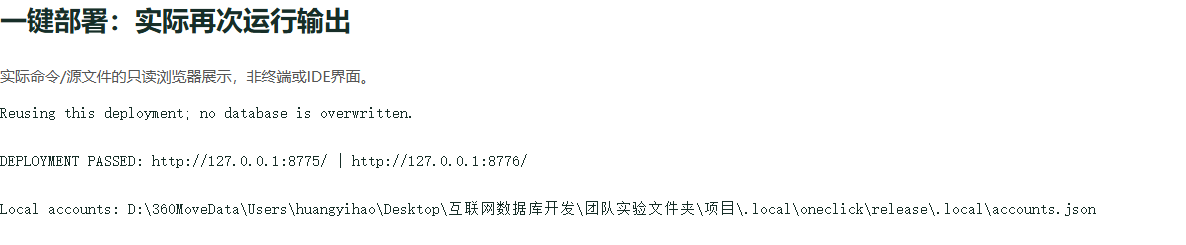
\includegraphics[width=\linewidth,height=.33\textheight,keepaspectratio]{../../figures/deployment.png}
\caption{一键部署实际运行结果}
\end{figure}

\begin{figure}[H]\centering
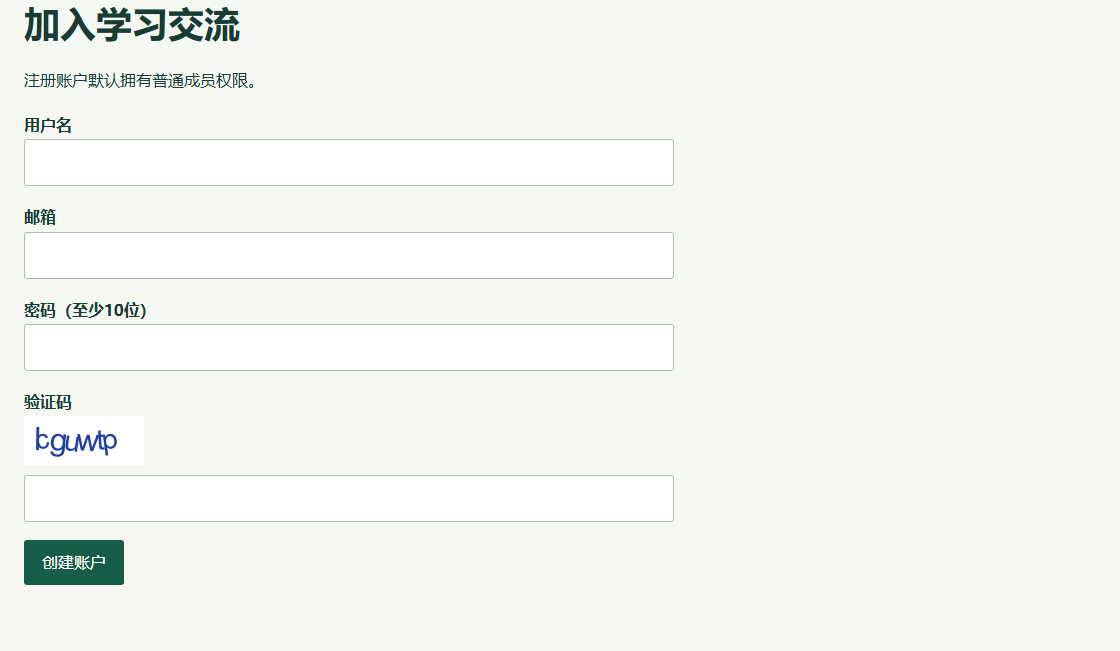
\includegraphics[width=\linewidth,height=.33\textheight,keepaspectratio]{../../figures/signup_captcha.png}
\caption{注册验证码}
\end{figure}
\section{主要代码节选}
下载文件的目录边界与摘要检查如下，来源为项目实际Model。
\VerbatimInput[fontsize=\scriptsize,breaklines=true,breakanywhere=true,firstline=12,lastline=22]{../../app/common/models/AssignmentFile.php}

\end{document}
